\chapter{多重化プログラミング}
\section{多重化プログラミングとは}
複数のプログラムを一つのコンピュータで処理することを多重化プログラミング
という。文書作成ソフトを起動している間にもメールソフトは一定の間
隔でサーバーに新着メールが届いているかを確認するように設定できる。これは
複数のプログラムが平行して処理している一例にすぎない。最近のCPUはマルチ
コアなので本当の意味で複数のプログラムを並行して処理ができる。

最近のOSではプログラムの実行単位をプロセスと呼び、いくつかのリソースから
構成される。それリソースは他のプロセスから独立しており互いに直接に参照で
きない。プロセス間でデータを交換するための機能としてプロセス間通信がOSで
用意している。

最近のOSではプロセスの中で並行処理が可能となるスレッドが提供されている。
スレッドはプロセスとは異なり、スレッド間でデータを共有することが可能であ
る。共有されるデータの書き込みに関しては複数のスレッドから同時に書き込み
が起きないようにするなどの注意が必要であり、OSはそのような環境を提供して
いる。
\section{Ajaxによる並行処理}
Ajax を用いてサーバーに同時に複数のデータを要求することも可能である。サー
バーがそれらの要求を並行処理するのであればデータ処理の効率化ができる
\footnote{PHPをサーバーモードで起動すると並行処理は行われないようである。
XAMPPでは並行処理が行われる。}。
\begin{Exec}\upshape\label{contPrimes}
 次のリストは$10,000,000$以下の素数を$1,000,000$ずつの区間に分けてサーバー
 に要求するものである。

 図\ref{countPrimes-Ajax-start}はこのWeb ページの初期画面である。
 \begin{figure}[ht]
	\begin{center}
	 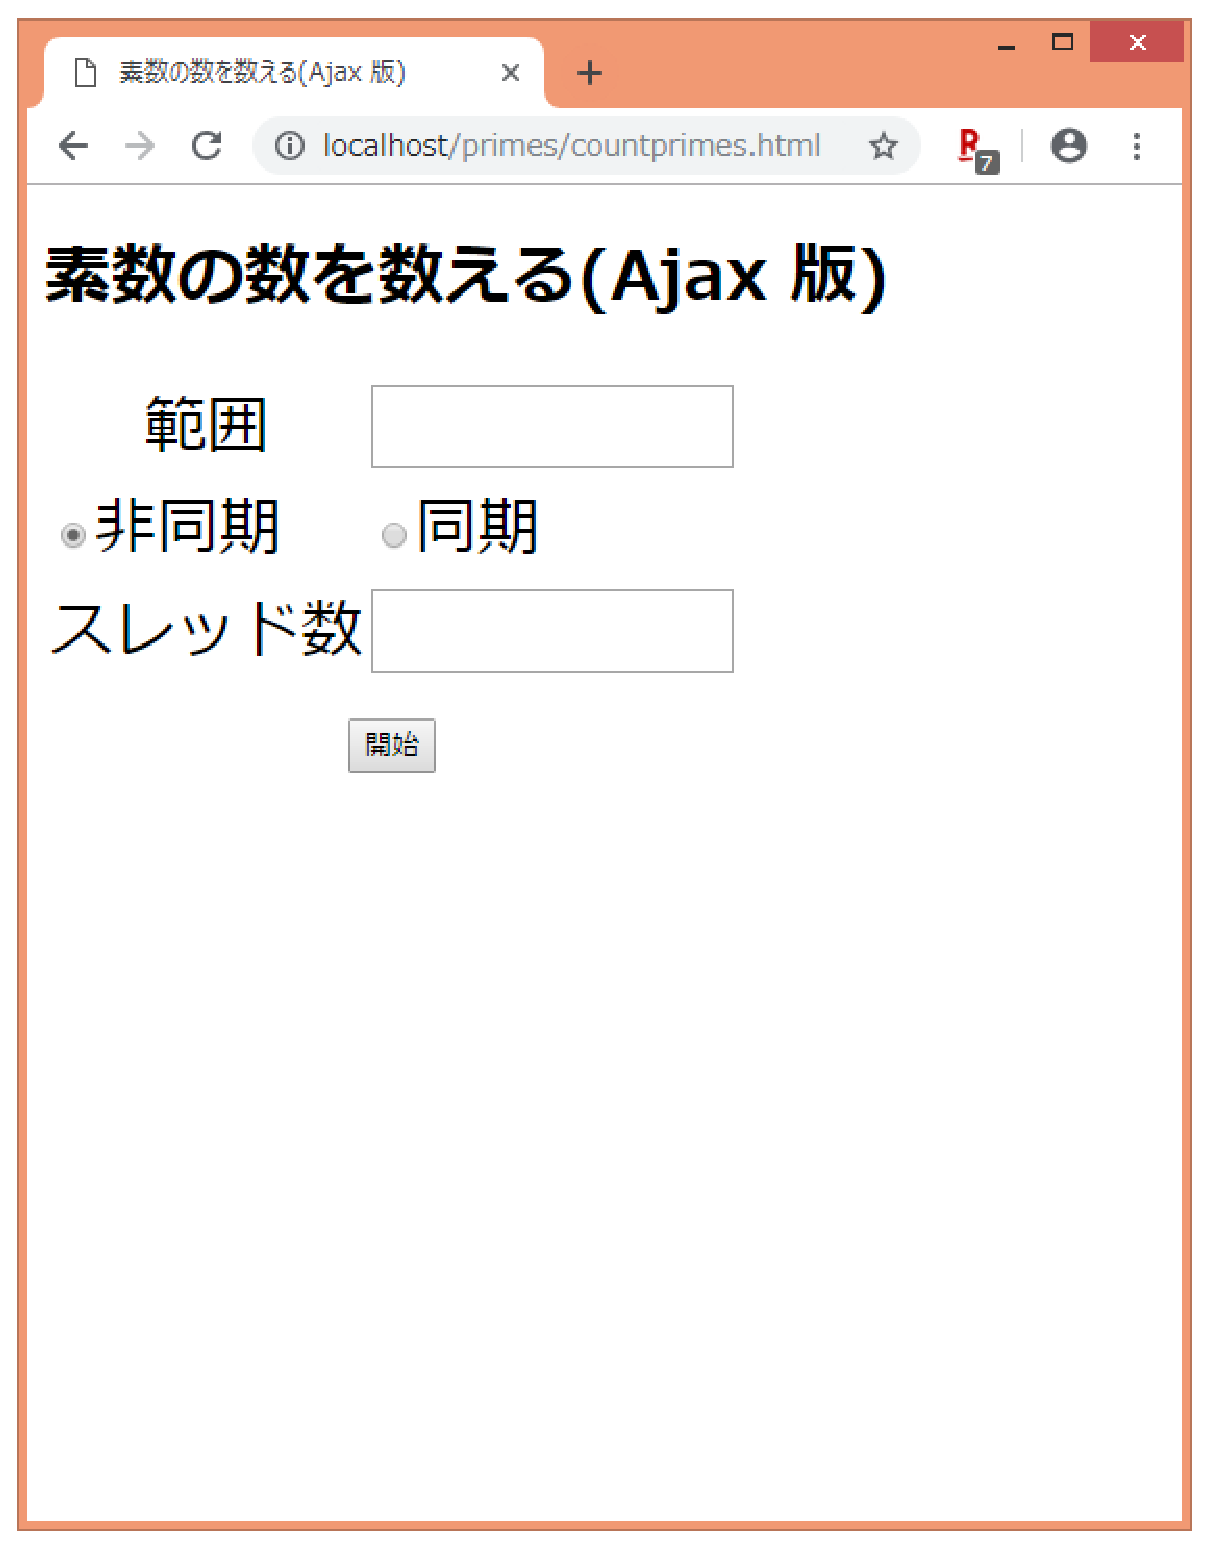
\includegraphics[width=0.5\textwidth]{primes/countPrimes-start.eps}
	\end{center}
 \caption{素数の数を数える(Ajax版)開始画面}\label{countPrimes-Ajax-start}
 \end{figure}

 素数の数を求める範囲と、Ajaxを実行するモード、求める区間の分割数と実行
 開始の美単が並んでいる。

図 \ref{countPrimes-Ajax-res}は求める範囲を$10,000,000$、分割を $10$に設
 定し、非同期モードで起動したことに結果画面である。
 \begin{figure}[ht]
	\begin{center}
	 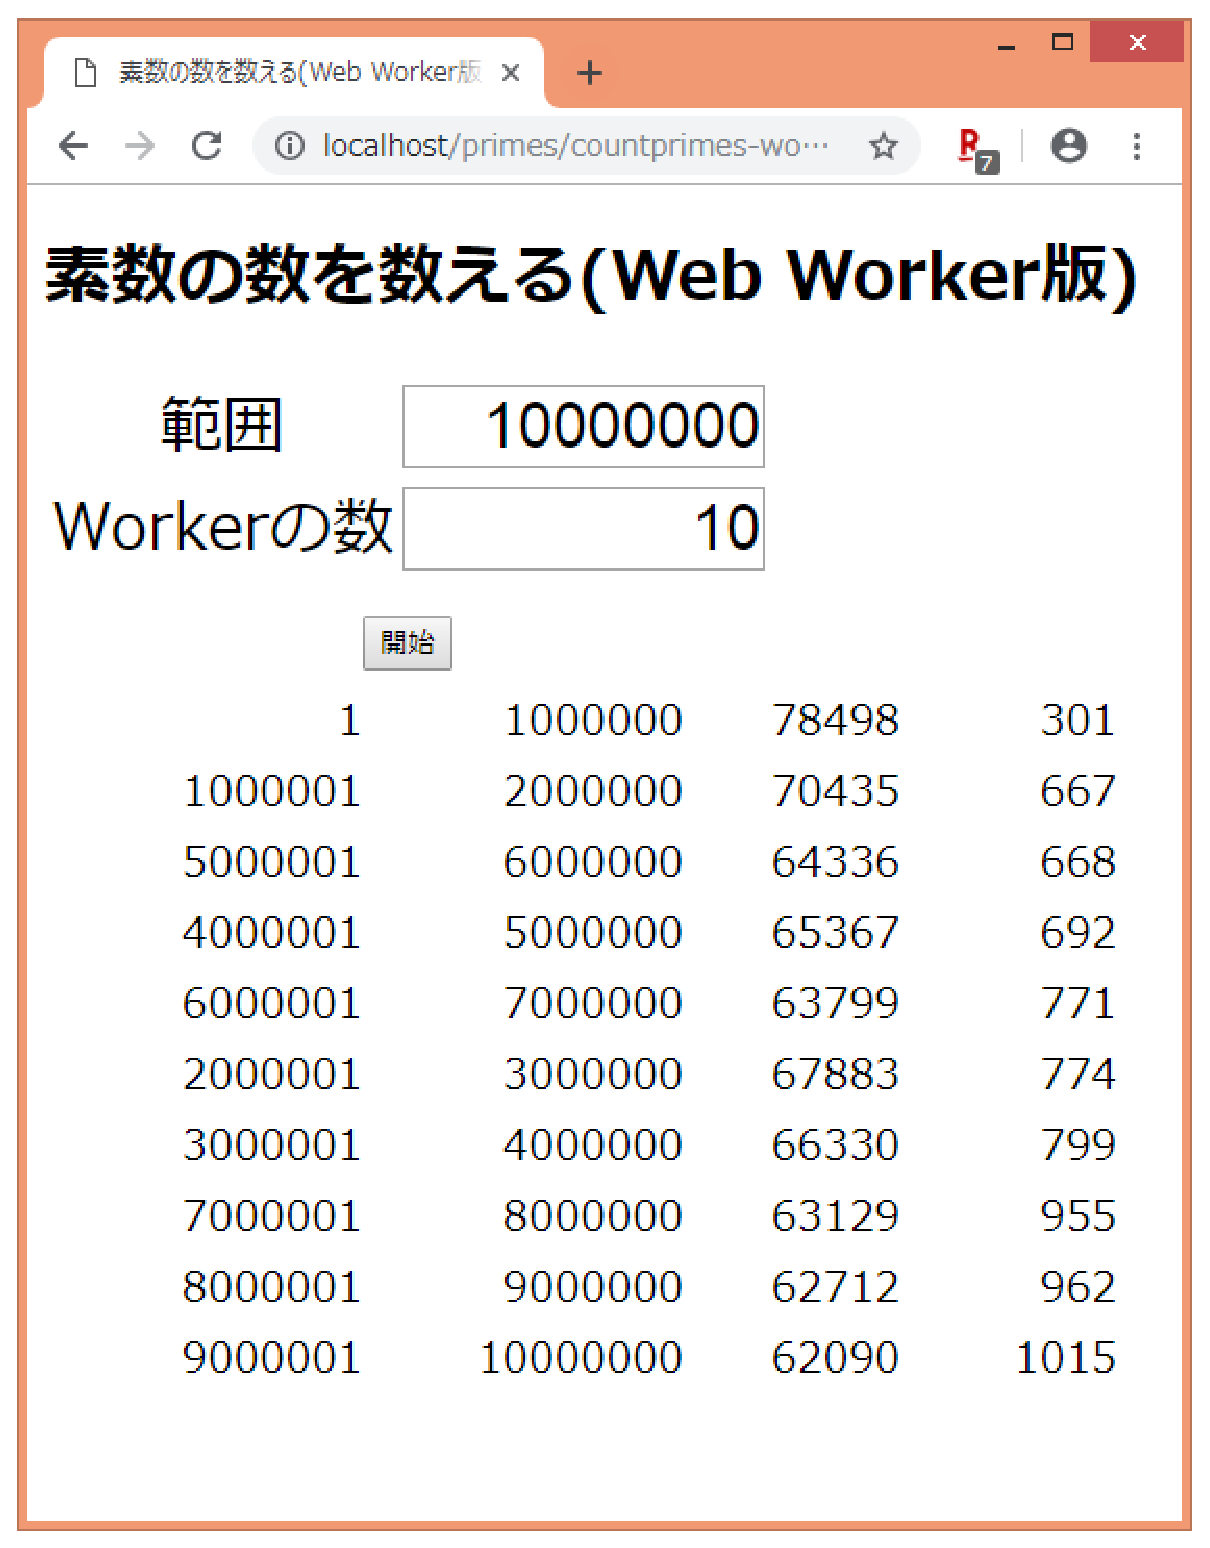
\includegraphics[width=0.5\textwidth]{primes/countPrimes-res.eps}
	\end{center}
 \caption{素数の数を数える(Ajax版)計算結果画面}\label{countPrimes-Ajax-res}
 \end{figure}

 項目は左から区間の下限と上限、その区間に含まれる素数の数、開始時間からその区間の実行
 終了までの時間(ミリ秒単位)である。
 
 次のリストは計算の起動と、結果を表示するWebページのものである。
 \LISTN{../primes/countPrimes.html}{1}{last}{\normalsize}
 \begin{itemize}
  \item 5行目で Ajax を用いてサーバーへの要求と結果を処理するJavaScriptっ
        ファイルを読み込む。
  \item 6行目でこのページに適用されるスタイルシートの読み込む。
  \item 13行目から16行目で素数の個数を求める範囲を指定するテキストボック
        スを配置している。
  \item 17行目から20行目でAjaxを起動するモードの指定をするラジオボタンを
        配置している。
  \item 21行目から24行目で同時に発行するAjaxの要求の個数を指定するテキストボック
        スを配置している。
  \item 25行目から29行目で計算開始するボタンを配置している。
 \end{itemize}
 次のリストは前のhtmlファイルで読み込まれるcssファイルの内容である。
 \LISTN{../primes/primes.css}{1}{last}{\normalsize}
 \begin{itemize}
  \item 1行目から4行目はテキストボックスに適用される。このページのテキス
        トボックスは数が入力さっるので、文字列を右寄せに(2行目)している。
  \item 5行目から7行目では\texttt{table}要素内の\texttt{td}要素の文字の
        大きさを指定している。 
  \item 8行目から12行目では素数の個数を表示する\texttt{table}要素ないの
        \texttt{td}要素の文字の位置(9行目)、文字の大きさ(10行目)と表示幅
        (11行目)を指定している。
  \item 13行目から15行目では右2つの\texttt{td}要素の幅を前の2つと異なる
        値に設定(\texttt{100px})している。
 \end{itemize}
 次のリストはAjaxを処理するためのJavaScriptファイルである。
 \LISTN{../primes/countPrimes-Ajax.js}{1}{last}{\normalsize}
 \begin{itemize}
  \item 2行目と3行目で\texttt{form}要素と結果を表示するための
        \texttt{table}要素を得ている。
  \item 4行目ではAjaxを非同期と同期モードの切り替えのラジオボタンを「非
        同期」に設定している。
  \item 6行目から44行目は「開始」ボタンが押されたときの処理を記述してい
        る。
        \begin{itemize}
         \item 6行目ではボタンの操作ができないようにしている。
         \item 7行目から9行目は結果を表示している内容を消去するために、
               表示する要素である\texttt{table}要素を取り除き(7行目)、そ
               の要素だけのコピー(子要素はなし)を作成(8行目)てそれを再び、
               子要素として登録(9行目)している。
         \item 10行目から11行目では素数を求める範囲を最低で$10^{6}$にな
               るようにしている。
         \item 12行目から13行目では区間を分ける数を設定している。
         \item 14行目では個々の処理で求める範囲の幅を求めている。
         \item 15行目ではその時点での時間を求めている。
         \item 16行目では発行したAjax通信の数を管理する変数を初期化して
               いる。
         \item 17行目から41行目で指定された個数分のAjax通信を発行してい
               る。
         \item 18行目から34行目ではAjax通信オブジェクトを作成している。
               作成が成功したのならば(35行目)発行した通信の数を一つ増や
               し(36行目)、通信を開始する(37行目から38行目)。
         \item 20行目から32行目はサーバーからのデータ処理の部分である。
         \item 20行目から21行目で表示1行分の要素\texttt{tr}を追加してい
               る。
         \item サーバーから送られてくるデータはJSON形式なのでそれを
               JavaScriptのオブジェクトに直し(22行目)ている。
         \item そのオブジェクトにボタンが押されてからの経過時間を追加(23
               行目)している。
         \item 24行目から28行目ではキーのリストを求め
               (\texttt{Object.keys()})、それらを順に\texttt{td}要素の中
               に表示している(25行目から27行目)。
         \item 28行目では発行したAjax通信の数を減らし、その値が$0$になっ
               たら「開始」ボタンが再び押せるようにしている
               (30行目から32行目)。
        \end{itemize}
 \end{itemize}
 次のリストはAjax通信で呼び出されるサーバー側のプログラムである。
 素数の判定は小さい素数で割り切れるかで行っている\footnote{ここでは非同期で処理
 が行われる例を出すために、素数の判定に関しては単純な方法を採用している。
 エラトステネスの篩を用いると処理速度は向上する。}。
 \LISTN{../primes/countPrimes.php}{1}{last}{\normalsize}
 \begin{itemize}
  \item PHPファイルをコマンドプロンプトからデバッグできるように、処理の
        ためのパラメータの処理を行っている(2行目と3行目)。スーパーグロー
        バル変数\Verb+$_GET+に指定したキーがあればそれを使用し、なければ
        コマンドラインの引数を格納する変数\Verb+$argv+をその値としている。
  \item 4行目では保存する素数の上限の値を設定し、その値を変数
        \Verb+$primes+に配列として格納する。この変数は5行目で初期化され
        ている。
  \item 6行目から15行目で残りの素数を求めている。ある数\Verb+$i+がその数
        の平方根以下の素数で割り切れないのならば素数と判定できる(10行目)。
  \item 16行目以下が与えられた区間における素数の個数を求める部分である。
  \item 開始の値が小さい場合には\Verb+$limit+以降から探し、素数の個数を
        \Verb+count($primes)+に初期化する(18行目から21行目)。
  \item 開始の値を奇数に設定し(22行目)、最後の値を求める(23行目)
  \item 26行目から35行目で与えられた区間の奇数が素数であるかの判定を行っ
        ている。この部分は小さい素数を求める部分と同じアルゴリズムである。
  \item 17行目、24行目36行目でクライアント側に送るデータを作成している。
  \item 37行目ではその結果をJSON形式に変換して、クライアント側に送ってい
        る。
 \end{itemize}
\end{Exec}
\section{Web Worker}
\iffalse
ブラウザにおけるJavaScriptの処理はどこか一か所しか実行されない。これによ
りあるイベントが処理されている間は他のイベントの処理が行われないのでプロ
グラムのアルゴリズムが簡単になる。一方、最近のCPUではマルチコアが標準と
なり、複数の処理を同時に行うことは当たり前となっている。

並行処理を行う方法としては独立したプログラム(プロセス)を用いる方法と、単一のプログ
ラム内でスレッドと呼ばれる実行単位を起動して行う方法がある。
独立したプログラムで行う場合にはそれぞれのプログラムがデータを個別に持つ
ので共通のデータを必要な時に渡したり、参照し
たりする機能を効率よく行う必要がある。

一方、スレッドはあるプログラム内で起動され、元のプログラムと同じメモリーっ
空間を共有するために、データの受け渡しをしなくてもよい。
\fi
ブラウザにおける
JavaScriptで並行処理を行う機能を提供するものとしてWeb Workerオブジェクト
が提案されている
\footnote{\texttt{https://developer.mozilla.org/en-US/docs/Web/API/Web\_Workers\_API/Using\_web\_workers}\label{webworkers}}
。
Workerオブジェクトは呼び出されるプログラムとは別のメモリー空間で実行され、
元のプログラムとのデータ交換はメッセージの通知というイベントを通じて行う。
したがって、Web Workers はプロセス間通信に似た環境を提供しているといえる。

この節では前節の素数の数を求めるプログラムをWeb Worker を用いて書き直し
 たものを紹介する。

 なお、このプログラムをエクスプローラーからダブルク
 リックして起動する(URLが\texttt{file:}で始まる)と、ブラウザによって
 は\texttt{Worker}が起動できないことがある。その場合にはローカルにサーバー
 を起動し、必要なファイルをドキュメントルートにコピーすればよい。
 \pageref{webworkers}ページの脚注\ref{webworkers}にあるブラウザに関する互換
 性の部分を参照のこと。

   \begin{Exec}\upshape
    図\ref{countPrimes-workers-res}はWeb Workers を利用して素数を求める
    Webページの結果画面である。
    \begin{figure}[ht]
	\begin{center}
	 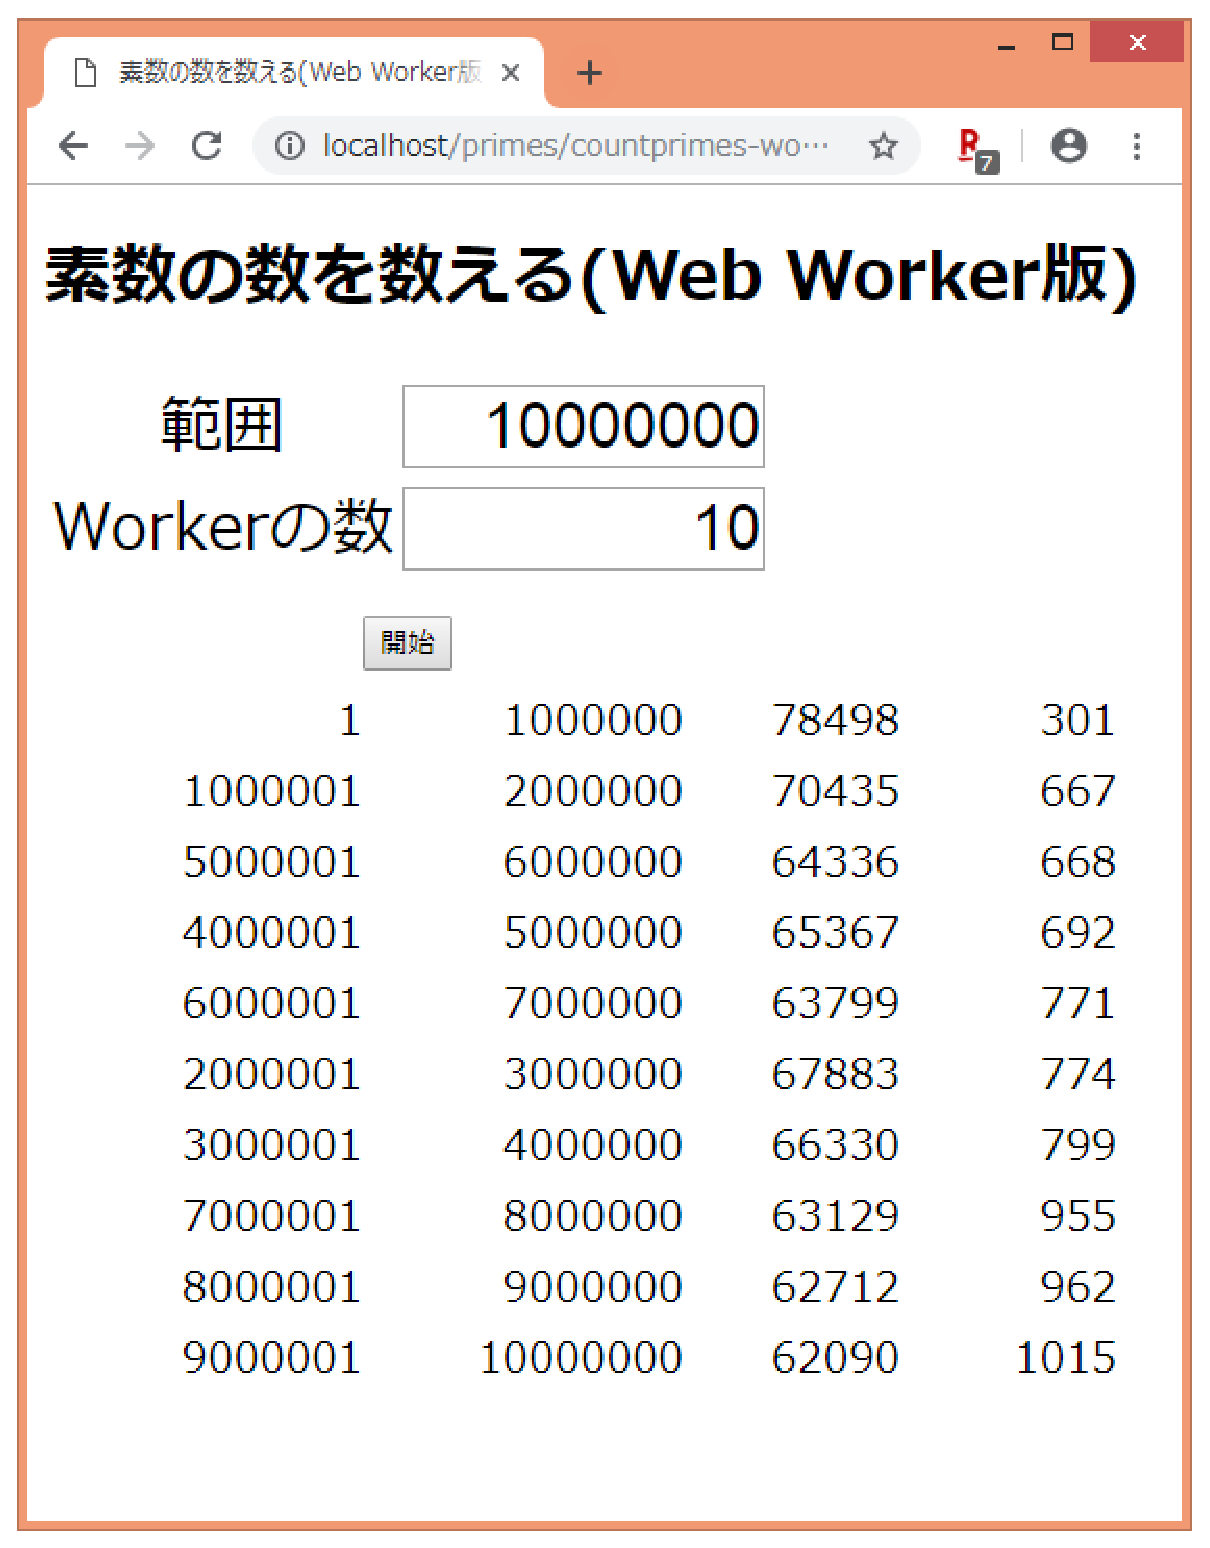
\includegraphics[width=0.5\textwidth]{primes/countPrimes-workers-res.eps}
	\end{center}
 \caption{素数の数を数える(Web workers版)計算結果画面}\label{countPrimes-workers-res}
 \end{figure}

    計算結果の順がばらばらで、計算速度も速いことが分かる。
    
 次のリストはWeb Worker版の素数の数を求めるHTMLファイルである。
 \LISTN{../primes/countPrimes-workers.html}{1}{last}{\normalsize}
 以前のも のからラジオボタンの部分がないものとなっている。当然のことなが
 ら読み込まれるJavaScriptファイルも異なっている。

 次のリストは読み込まれるJavaSCriptファイルである。
 \LISTN{../primes/countPrimes-workers.js}{1}{last}{\normalsize}
 Ajax通信のときと比較できるようにできるだけ同じプログラムの流れとなって
 いる。
 \begin{itemize}
  \item 13行目まではAjaxのときと同じである。
  \item 17行目から20行目で必要な個数のWeb Workerオブジェクトを作成してい
        る。Web Workerオブジェクトは\Verb+Worker+コンストラクタで作成す
        る。この引数には処理をするJavaScriptファイルを指定する。
  \item Workerオブジェクトにデータを送るメソッドが\ElmJ{postMessage}であ
        る。引数としてはJavaScriptで扱えるデータを用いる。ここではオブジェ
        クトを与えている。
  \item Workerからのメッセージは\Verb+onmessage+イベントを通じて受け取る
        ことができる。この引数は\Verb+message+オブジェクトであり、その
        \Verb+data+プロパティが送られてきたデータとなる(26行目)。
  \item データが送られてきたので\Verb+worker+の動作を停止し(35行目の
        \Verb+terminate+メソッド)、オブジェクトを消去する(36行目)。
 \end{itemize}
 \Verb+worker+オブジェクトに再びメッセージを送れば再度処理をさせることが
 できる。

 次のリストは\Verb+worker+の処理をするJavaScriptのプログラムである。
 \LISTN{../primes/primes.js}{1}{last}{\normalsize}
 \begin{itemize}
  \item 1行目の\Verb+self+は\Verb+Worker+のもととなるオブジェクトを指す。
        こので\Verb+onmessage+イベントの処理のプログラムを登録する。
  \item 処理内容は全く前と同じである。workerが2回目以降呼び出されたかど
				うかを記憶する変数(2行目の変数\texttt{Status})を利用して2回目以
				降の呼び出し時には素数のリストを再度作成しないようにするためにい
				くつかの変数をイベント処理関数の外で定義している(1行目から3行目)。
  \item 最後に\ElmJ{postMessage}メソッドを用いて呼び出し元にデータを送信
        する(39行目から40行目)。
 \end{itemize}
\end{Exec}
 \begin{Prob}\upshape このリストについて次のことを行いなさい。
  \begin{enumerate}
   \item 実行するごとに結果の並びや計算終了時間が変化すること。
   \item スレッドの個数を変えると表示する区間が変化すること。また、どの
         場合が一番実行時間が短いかを調べる。
   \item 計算結果が戻ってきた順に区間の上限と下限やその
 区間の素数の個数が表示される。素数の区間が小さい方から大きい方に並ぶよ
 うにプログラムを直す。
   \item 同時に起動する\texttt{worker}の数を減らして、一つの処理が終わっ
         た時に別の区間の処理を与えるようにプログラムを直す。たとえば、区間は10に
         分けるが、生成する\texttt{worker}は3つにするように指定でき
         るようにする。
  \end{enumerate} 
 \end{Prob}
 \section{\texttt{pthread}による多重化}
 この節ではUnixで標準のスレッド処理をする\texttt{pthread}ライブラリーを
  用いで今までの素数を求めるプログラムを書き直したものを示す\footnote{こ
  のプログラムの実行はWindowsでUnix互換環境を提供するCygwinの上で実行し
  ている。}。
	次のリストは必要なヘッダーファイルの読み込みを行っている。
  \LISTN{../primes/countPrimes-simple-pthread.c}{1}{4}{\normalsize}
	4行目で\texttt{pthread}ライブラリを使用するために必要な
  \texttt{pthread.h}を読み込んでいる。

	次のリストは必要な定数を定義している。
  \LISTN{../primes/countPrimes-simple-pthread.c}{6}{9}{\normalsize}
	9行目で最大のスレッド数を10に制限している。

	次のリストはスレッドから参照する変数を定義している。
  \LISTN{../primes/countPrimes-simple-pthread.c}{11}{13}{\normalsize}
	初めの2つの素数を素数のリストに定義し(12行目)、素数のリストにある素数
  の数(\texttt{ic})と区間の幅(\texttt{Step})を定義している。

	次のリストは小さい素数のリストを求めるものである。
  \LISTN{../primes/countPrimes-simple-pthread.c}{15}{29}{\normalsize}
	JavaScriptのときと同様のアルゴリズムで作成している。
  戻り値はリストにある素数の数である。

	次のリストはスレッドを構成する関数を定義している。
  \LISTN{../primes/countPrimes-simple-pthread.c}{30}{47}{\normalsize}
	\begin{itemize}
	 \item 	\texttt{pthread}ライブラリーではスレッドとして呼び出される関数の戻り値
  は\texttt{void *}に限られている。ここでは戻り値はなく、求めた結果はス
  レッド内で出力している(46行目)。
	 \item スレッドで呼び出される関数の引数も\texttt{void *}である必要があ
				 る。複数のパラメータを渡すときには構造体にして、そのポインタを
				 渡すことになる。
	\end{itemize}

	次のリストは
  \LISTN{../primes/countPrimes-simple-pthread.c}{49}{last}{\normalsize}
